
\part{Préparer une partie}

\section{Construire votre Liste d'Armée}
\label{building_an_army}

Batailles Fantastiques : Le 9\ieme{} Âge propose une série de Livres d'Armée qui décrivent les spécificités de chaque armée. Chaque armée regroupe un ensemble unique de personnages, troupes et règles. Les \textbf{Personnages} sont répartis entre Seigneurs et Héros, et les \textbf{Troupes} entre unités de Base, unités Spéciales et unités Rares.

\noindent\hspace*{\fill} \begin{minipage}[t]{0.3\textwidth}
\begin{center}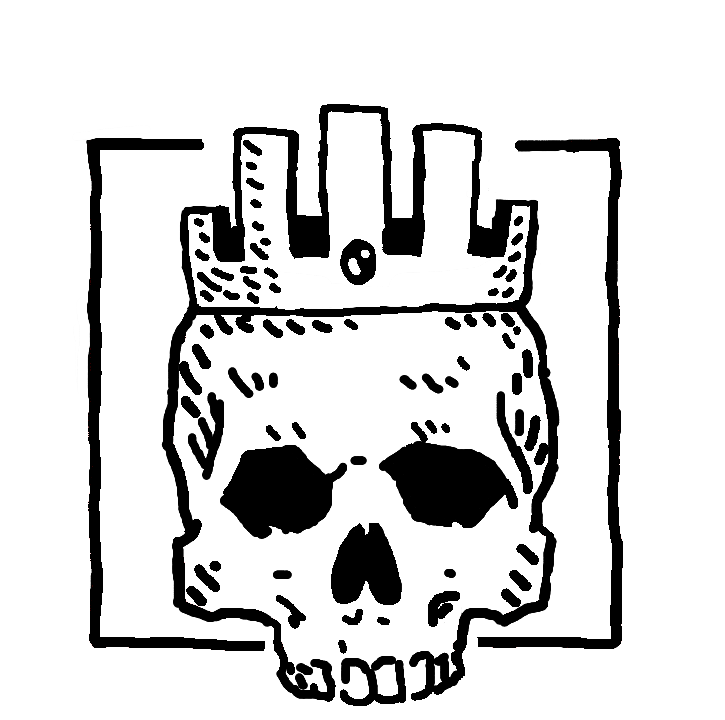
\includegraphics[width=2.5cm]{../Layout/pics/logo_lord.png}

Les Seigneurs sont les individus les plus puissants d'une armée.
\end{center}
\end{minipage}\hspace*{1cm}
\begin{minipage}[t]{0.3\textwidth}
\begin{center}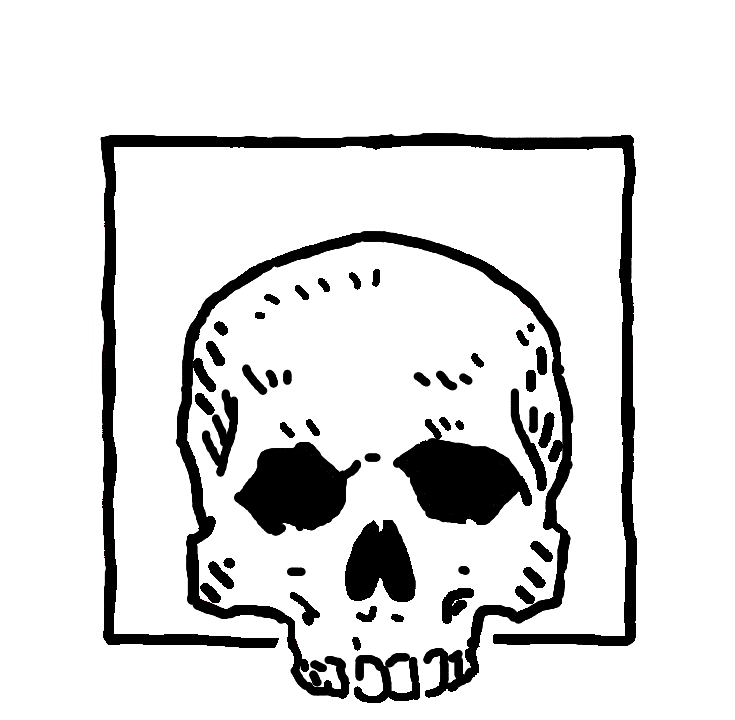
\includegraphics[width=2.5cm]{../Layout/pics/logo_hero.png}

Les Héros sont des individus exceptionnels.
\end{center}
\end{minipage}\hspace*{\fill}

\noindent\begin{minipage}[t]{0.3\textwidth}
\begin{center}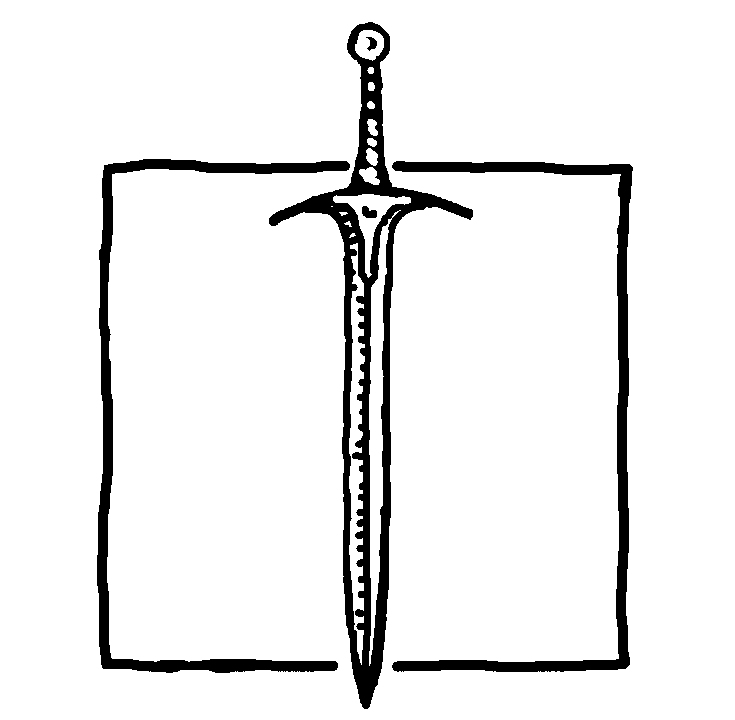
\includegraphics[width=2.5cm]{../Layout/pics/logo_core.png}

Les unités de Base représentent les guerriers les plus communs de l'armée.
\end{center}
\end{minipage}\hfill
\begin{minipage}[t]{0.3\textwidth}
\begin{center}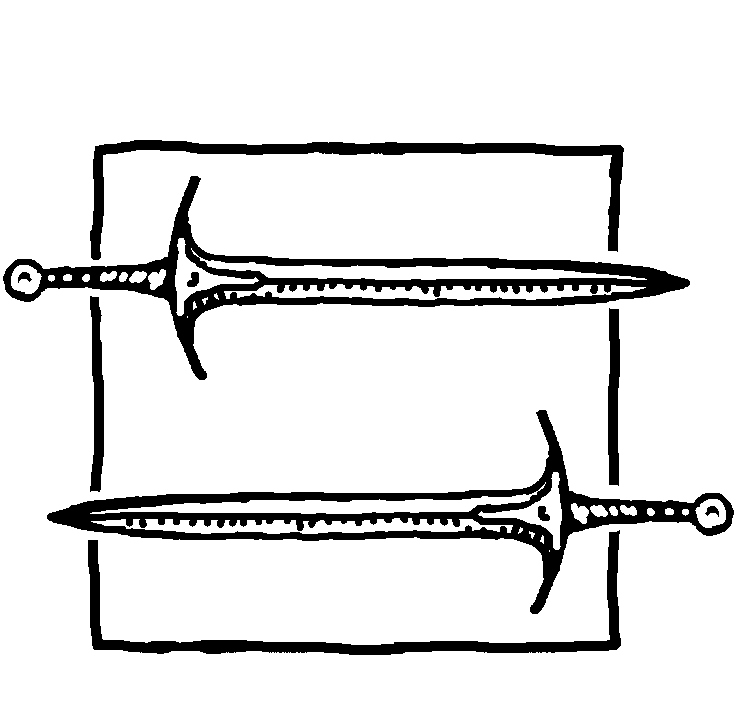
\includegraphics[width=2.5cm]{../Layout/pics/logo_special.png}

Les vétérans et régiments d'élite constituent les unités Spéciales.
\end{center}
\end{minipage}\hfill
\begin{minipage}[t]{0.3\textwidth}
\begin{center}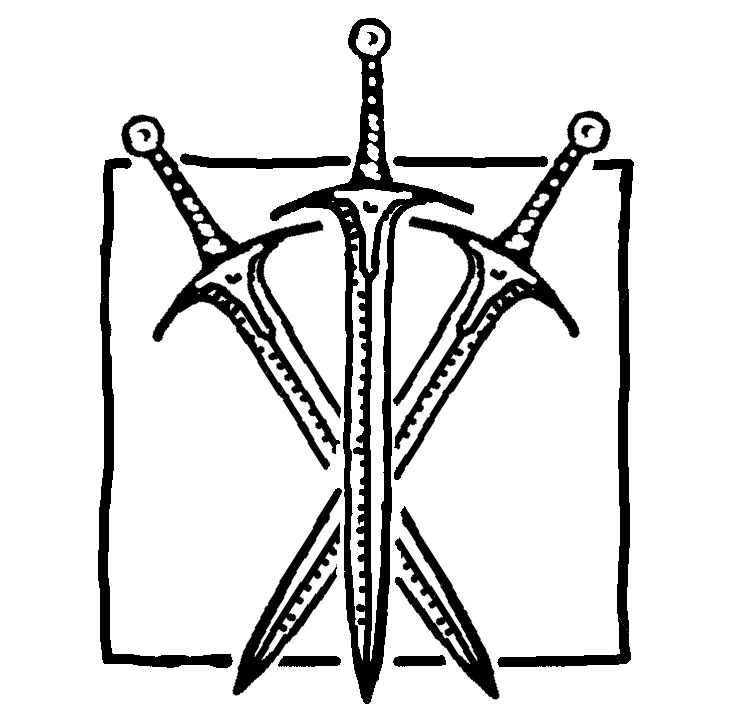
\includegraphics[width=2.5cm]{../Layout/pics/logo_rare.png}

Les unités Rares sont des troupes extraordinaires, des monstres peu communs et des machines de guerre inhabituelles.
\end{center}
\end{minipage}

\vspace*{10pt}
La première étape de la construction d'une armée est d'écrire un choix d'unités, leurs options et leurs Coûts en Points sur un document qu'on appelle \og Liste d'Armée \fg{}. La composition d'une liste est sujette à des règles et restrictions, que l'on décrit en détails dans la suite du chapitre.

\subsection{Coût en points}

Chaque unité, arme, amélioration, Objet Magique, etc. vaut un certain montant de points. Le Coût en Points d'une unité est la somme des Coûts en Points de chacune de ses figurines et des options. Le Coût en Points d'une armée est la somme des Coûts en Points de toutes ses unités.

\noindent\textbf{\newfromWHB{Demi-point}}

La valeur en point d'une unité doit être entière. Si une amélioration coûte 0,5 point, le coût final de l'unité est arrondi à la valeur supérieure.

\noindent\textbf{\newfromWHB{Coûts Seigneur / Héros}}

Si le coût d'une option ou d'un objet magique est écrit avec un \og / \fg{}, par exemple 50 / 40 pts, la première valeur est le coût pour un Seigneur tandis que la seconde s'applique pour un Héros ou un Champion.

\section{Restrictions}

Une armée de Batailles Fantastiques : Le 9\ieme{} Âge doit suivre des règles simples de composition, détaillées ci-dessous :

\begin{itemize}[label={\textbullet}]
\item \textbf{Coût en Points de l'armée}\newline
Le Coût en Points de l'armée, combinant la valeur de toutes les unités, équipements et options, ne doit pas dépasser la limite en points décidée pour la partie. Elle peut cependant descendre jusqu'à 20 points en dessous de cette limite.

\item \textbf{Catégories d'unités}\newline
Les unités sont regroupées en 5 Catégories. Le nombre de points que l'on peut dépenser dans chaque groupe dépend de la Catégorie. De plus, une même entrée du livre d'armée ne peut être prise qu'un certain nombre de fois. Ces informations sont résumées dans la table \ref{table/unitcategories} ci-dessous.

\begin{table}[!htbp]
\centering
\begin{tabular}{rcc}
\hline
 & \textbf{Limite de points} & \textbf{Limite de duplication} 			\tabularnewline
\textbf{Base} 					& min. 25 \% 			& \newfromWHB{max. 4} 	\tabularnewline
\textbf{Spécial} 				& - 					& max. 3 			\tabularnewline
\textbf{Rare} 					& max. 25 \% 			& max. 2 			\tabularnewline
\textbf{Héros} 					& max. \newfromWHB{50 \%} 	& \newfromWHB{max. 3} 	\tabularnewline
\textbf{Seigneurs} 			& max. \newfromWHB{35 \%} 	& \newfromWHB{max. 3} 	\tabularnewline
\textbf{Héros + Seigneurs} & max. 50 \% 			& - 				\tabularnewline
\hline
\end{tabular}
\caption{\label{table/unitcategories}Restrictions de composition d'armée.}
\end{table}

\newfromWHB{Parfois, certaines unités peuvent être déplacées d'une Catégorie à une autre. Par exemple, certaines règles peuvent autoriser un joueur à prendre un Char comme choix de Base plutôt qu'en choix Spécial. Dans de tels cas, il faut respecter à la fois la limite de duplication de son ancienne Catégorie et de sa nouvelle. La limite de points compte, quant à elle, seulement dans la nouvelle catégorie. Dans notre exemple précédent, vous ne pouvez pas inclure plus de 3 Chars dans votre armée, mais ceux-ci compteront dans les 25 \% d'unités de Base nécessaires.}

\item \textbf{Taille d'armée minimale}\newline
\newfromWHB{Une armée doit contenir au moins 4 unités sans compter les Personnages. On ne peut comptabiliser qu'une seule unité de type Machine de Guerre pour atteindre ce minimum.}
\item \textbf{Le Général}\newline
Un des Personnages de l'armée doit être nommé Général. Il faut donc qu'il y ait au moins un Personnage dans l'armée capable de tenir ce rôle. Une armée ne peut comporter qu'un seul Général.
\item \textbf{\newfromWHB{\oneofakind{} et \oneperarmy}}\newline
Les unités, options et objets marqués \oneofakind{} ou \oneperarmy{} ne peuvent être pris qu'une fois par armée. Ceux marqués \oneofakind{} peuvent être pris en deux exemplaires dans une Grande Armée.
\item \textbf{\newfromWHB{\zerotoXchoice{X}}}\newline
Certaines unités disposent d'une limite de duplication différente notée \zerotoXchoice{X}, par exemple \zerotoXchoice{2}. Cela signifie que ces unités peuvent être prises entre 0 et X fois, en ignorant les limites de duplication classiques. La limite maximale X est divisée par 2 pour une Patrouille en arrondissant à l'unité supérieure, et multipliée par 2 pour une Grande Armée.
\end{itemize}

\newpage
\section{Patrouilles et Grandes Armées}

Les règles de composition d'armée peuvent être modifiées selon la limite en points de la partie, si les armées sont plus petites ou grandes que la norme.

\begin{multicols}{2}\raggedcolumns

\begin{center}\textbf{\newfromWHB{Patrouilles}}\end{center}

Les armées de 1500 points ou moins sont appelées Patrouilles. La taille d'armée minimale est réduite à 3 unités. La table suivante donne les nouvelles limites de duplication :

\begin{center}
\begin{tabular}{rp{3.8cm}}
\hline
\textbf{Base} 							& max. 2 \tabularnewline
\textbf{Spécial} 						& max. 2 \tabularnewline
\textbf{Rare} 							& max. 1 \tabularnewline
\textbf{Héros et Seigneurs}	& max. 2 \tabularnewline
\textbf{\oneofakind}			    & max. 1 \tabularnewline
\textbf{\oneperarmy}				& max. 1 \tabularnewline
\textbf{\zerotoXchoice{X}} 	& divisée par 2,\newline arrondie au supérieur \tabularnewline
\hline
\end{tabular}
\end{center}

\columnbreak

\begin{center}\textbf{\newfromWHB{Grandes Armées}}\end{center}

Les armées de 4000 points ou plus sont appelées Grandes Armées. Les unités marquées \oneofakind{} peuvent être prises en deux exemplaires. La table suivante donne les nouvelles limites de duplication :

\begin{center}
\begin{tabular}{rl}
\hline
\textbf{Base} 							& max. 8 \tabularnewline
\textbf{Spécial} 						& max. 6 \tabularnewline
\textbf{Rare} 							& max. 4 \tabularnewline
\textbf{Héros et Seigneurs}	& max. 6 \tabularnewline
\textbf{\oneofakind}			    & max. 2 \tabularnewline
\textbf{\oneperarmy}				& max. 1 \tabularnewline
\textbf{\zerotoXchoice{X}} 	& doublée \tabularnewline
\hline
\end{tabular}
\end{center}
\end{multicols}

\newpage
\section{Liste d'Armée ouverte ?}

Les règles de ce jeu ont été équilibrées avec l'idée de listes d'armée complètement révélées. Par exemple, votre adversaire doit savoir quels Objets Magiques vos figurines possèdent. Nous encourageons les joueurs à partager leur Liste d'Armée complète avec leur adversaire au début de la partie, en détaillant unités, options, Objets Magiques, capacités spéciales, coûts en points, etc. Les seules choses qui ne doivent pas être montrées à votre adversaire sont celles explicitement citées comme cachées ou secrètes, comme par exemple dans quelle unité un Assassin est caché. Précisons que l'Assassin et son équipement sont quand même mentionnés dans la liste.

\subsection[Règles optionnelles pour listes cachées]{\newfromWHB{Règles optionnelles pour listes cachées}}
\label{hidden_lists}

Certains joueurs peuvent préférer jouer avec des listes dites \og cachées \fg{}. Rappelons que les règles du jeu n'ont pas été équilibrées dans cette optique. Dans ce cas, nous vous proposons de suivre les règles suivantes. La plus grande partie de votre armée doit rester connue de votre adversaire avant le début de la partie. Seuls quelques aspects sont secrets, ou \og cachés \fg{}. Les deux joueurs peuvent donner à leur adversaire une liste simplifiée dans laquelle les détails cachés sont omis.

Voilà les éléments qui peuvent être cachés : 

\begin{itemize}[label={-}]
\item Les Objets Magiques pris dans la liste commune de ce livre.
\item Les Objets Magiques spécifiques aux Livres d'Armée ainsi que toute option suivant les règles des Objets Magiques, comme les Objets Démoniaques et les Runes Naines.
\end{itemize}

Le reste doit être présenté dans la partie ouverte de votre liste. De plus, les Objets Magiques et assimilés qui ont un équivalent standard doivent être présentés sur la liste ouverte comme tels. Une Arme Lourde magique, par exemple, apparait comme une simple Arme Lourde.

Quand vous possédez au moins deux unités qui sont identiques dans la liste ouverte, mais qui ont une différence cachée, comme par exemple une Bannière Magique, vous devez avoir un moyen visible de les différencier, noté sur votre liste complète. Par exemple, la bannière rouge est la Bannière Magique, tandis que la bleue est ordinaire.

\noindent\textbf{Révéler les Objets Magiques}

Un Objet Magique, ou équivalent, doit être révélé à la première utilisation. Un objet est considéré comme utilisé quand il a une chance d'affecter le jeu d'une quelconque façon. Entre autres :
\begin{itemize}[label={-}]
\item si cela affecte un jet de dé, même si le résultat obtenu sur le dé ne déclenche pas d'effet ;
\item si cela altère une attaque, via une Arme Magique ou tout objet dont une règle affecte l'attaque ;
\item si cela altère un jet de sauvegarde. L'objet doit alors être révélé avant que les dés ne soient jetés. Remarquez qu'un objet qui affecte une sauvegarde de la même manière que son équivalent standard le ferait, comme un Bouclier Magique, ne doit pas forcément être révélé.
\end{itemize}

Un objet qui augmente la mobilité ne compte comme étant utilisé que lorsque l'unité se déplace plus loin qu'elle ne le pourrait sans l'objet, ou lorsqu'elle charge. Déclarez alors l'objet avant de lancer le jet de distance de charge, mais après que les réactions ont été déclarées. Pour les Objets Runiques Nains, ne révélez que la Rune qui est utilisée, pas la combinaison complète.

